% ------------ HEADER ------------ %


% PROJECT: Today I Learned Document
% AUTHOR: Miles Smith


% ------------ PREAMBLE  ------------ %


\documentclass[12pt]{article}
\usepackage{times}
\usepackage[margin=1.5in]{geometry}
\usepackage{amsmath,amsthm,amssymb}
\usepackage{graphicx}
\usepackage{multirow}
\usepackage{setspace}
\usepackage{subcaption}
\usepackage{caption}
\usepackage{float}
\doublespacing


% ------------ DOCUMENT ------------ %

\begin{document}

\begin{center}
\huge{\textbf{Today I Learned}}\\
\large{An insight into the fun things I am learning and doing}\\

\vspace*{0.5cm}
\textbf{Miles Smith}\\

\vspace*{1cm}
\textbf{Introduction}\\
\textit{In an attempt to better document the things that I am learning and help things stick with me, I am hoping to create this running document so I can ramble about whatever cool things I learn each day.}\\
\vspace*{2cm}
\clearpage

\end{center}

\section{Friday, March 11, 2022}

\par
What is the difference between Gauss's Law and Poisson's Equation for electrostatics? The big difference is that (in the differential form) Gauss's Law:

\begin{equation}
\centering
\nabla \cdot E = \frac{\rho}{\epsilon_0}
\end{equation}

is a general expression that should always be true. In contrast, Poisson's Equation assumes that there is no magnetic field (thus, it is electrostatic). This assumption states that 

\begin{equation}
\centering
\nabla \times E = 0,
\end{equation}

and subsequently,

\begin{equation}
\centering
E = - \nabla \phi,
\end{equation}

which can be substituted into Gauss's Law to give,

\begin{equation}
\centering
\nabla^2\phi = -\frac{\rho}{\epsilon}.
\end{equation}

Since it is based on an electrostatic assumption, Poisson's equation for electrostatics is not always true. 

\par
Anyway, to continue this seemingly lengthy discussion on ionic wind propulsion, one research group cited using a dielectric barrier discharge plasma, instead of a corona discharge plasma to reduce the applied voltage requirement. However, it seems like the DBD plasma might be less effective for high-speed airflow control, which is important for full-scale airplanes.  It might be useful for smaller, slower UAVs. I should add some sort of explanation on how a DBD plasma works, but I should spend this weekend learning about waves and studying for my finals on Monday and Tuesday. 

\section{Thursday, March 10, 2022}

\par
Today was the last day of classes for the winter quarter, which is an exciting and unsettling feeling. Will I be able to stay at Stanford and do a Ph.D. here? Will I go to MIT? Will I ever be able to schedule a meeting with Mark, Ted, and Erik? There is a bit of time to deal with this but really not a whole lot since I need to put together an application relatively soon. Nothing I can do about it tonight, but maybe I should bump Ted in the morning tomorrow. Anyway, today I learned a bit too much about Euler's identity, Euler's equations and trig properties to solve a single plasma physics problem.  As a note, Euler's identity says:

\begin{equation}
\centering
e^{i\pi} = -1, 
\end{equation}

and Euler's equation states that:

\begin{equation}
\centering
e^{i\theta} = \cos(\theta) + i \sin(\theta).
\end{equation}

By adding 

\begin{equation}
\centering
e^{i\theta} = \cos(\theta) + i \sin(\theta)
\end{equation} 

to 

\begin{equation}
\centering
e^{-i\theta} = \cos(-\theta) + i \sin(-\theta) = \cos{\theta} - i\sin(\theta)
\end{equation}

Euler's less intuitive relationships can also be derived which state that:

\begin{equation}
\centering
\cos(\theta) = Re(e^{i\theta}) = \frac{e^{i\theta}+e^{-i\theta}}{2}
\end{equation}

and

\begin{equation}
\centering
\sin(\theta) = Im(e^{i\theta}) = \frac{e^{i\theta} - e^{-i\theta}}{2i}
\end{equation}

The plasma wave table handout is also a blessing to help explain which types of waves will propagate in a plasma under a given set of conditions. I have much to learn about plasma waves I think. 

\section{Wednesday, March 9, 2022}

\par
An interesting article on Nature titled \textit{Flying with ionic wind} discussed how the ionocraft at MIT was developed. One of the big challenges with the ionocraft seems to be optimizing the weight so that the thrust from the corona is strong enough to create some lift.  This is probably why the scalability of the ionocraft is uncertain.  The original design was generated through some geometric parameter optimization algorithm to determine the optimal wing span and mass for the thrust generated.  One of the big challenges seems to be that takeoff is very hard and inefficient but once in flight the efficiency of ionic wind significantly increases making it more feasible. In their experiments, they reported an energy efficiency of only ~2\%, but it is believed that at high speeds the energy efficiency can be as high as 50\%. An interesting thing to note is that it can also be coupled with battery technologies to use electricity from batteries to possibly launch the plane and then use ionic wind propulsion as a secondary energy source.

\begin{figure}[H]
\centering
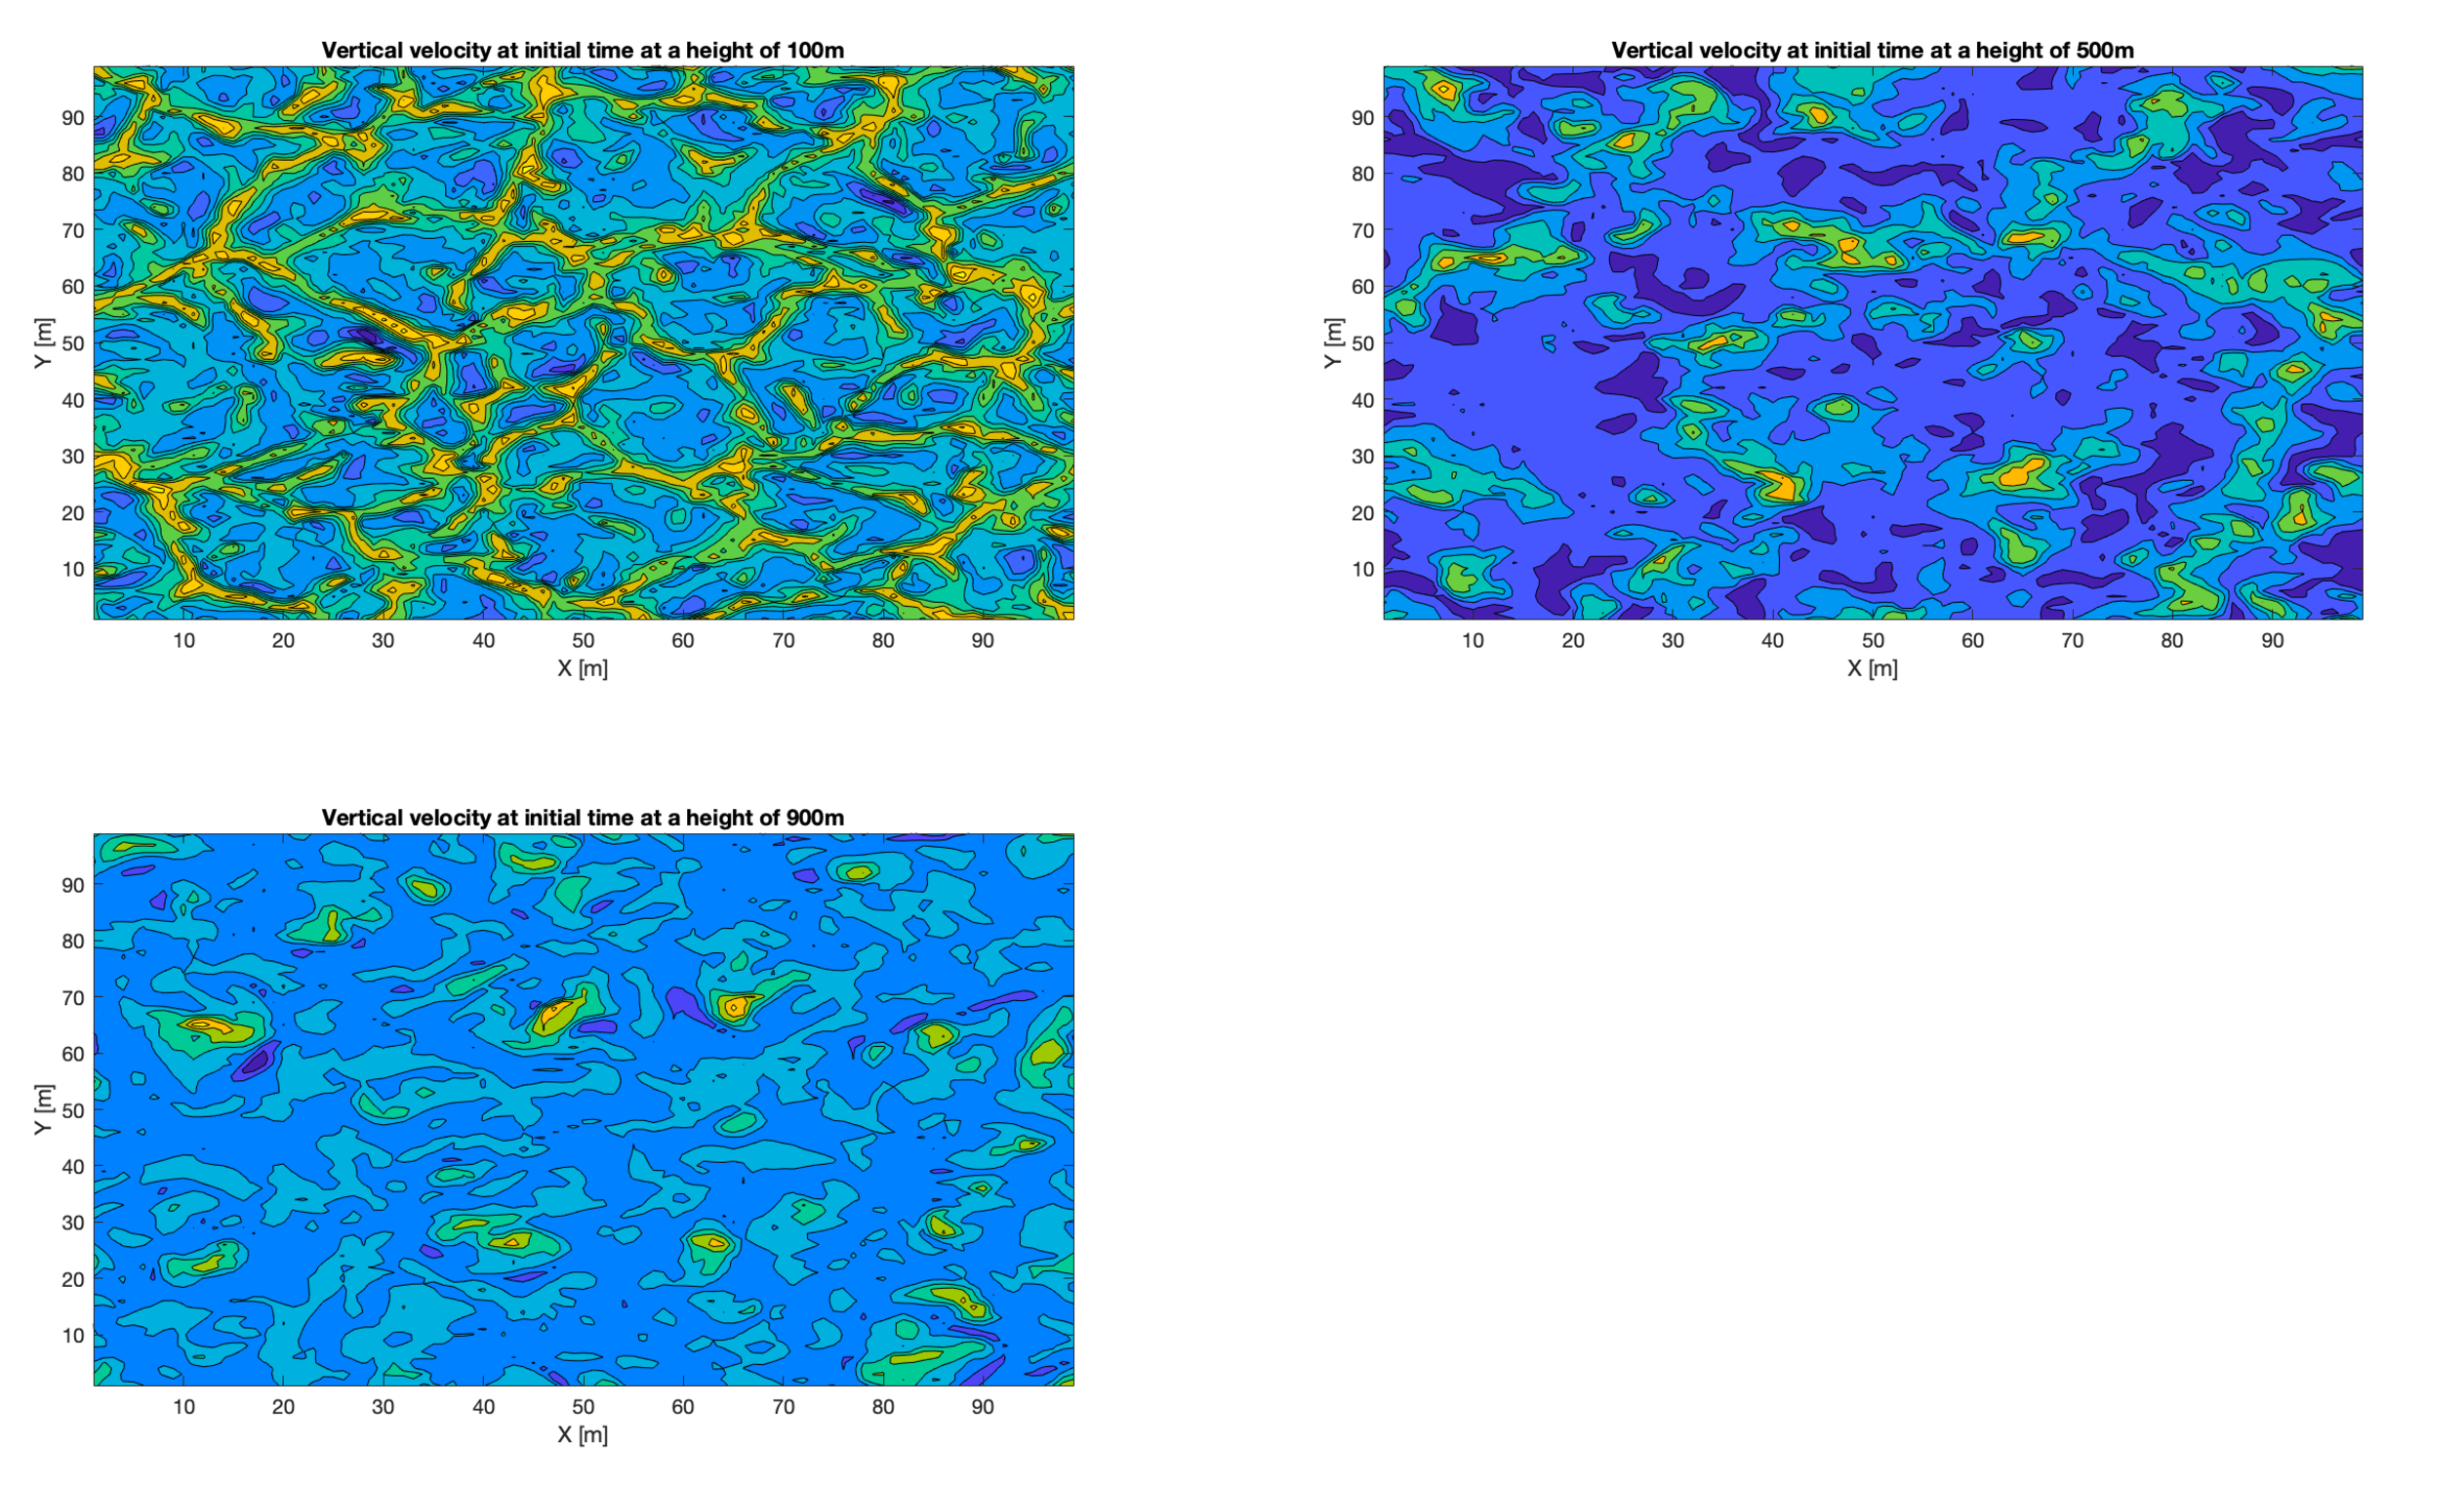
\includegraphics[width=\linewidth]{images/vertical_velocity_contour.pdf}
\end{figure}

\par
In Physics of Wind I am still looking at the large eddy simulations of a "quasi-steady free-convection ABL" that we can allegedly assume is horizontally homogeneous and does not evolve much temporally. Here are some interesting figures of how the vertical velocity profile changes (at the initial time) with height in the ABL.

\begin{figure}[H]
\centering
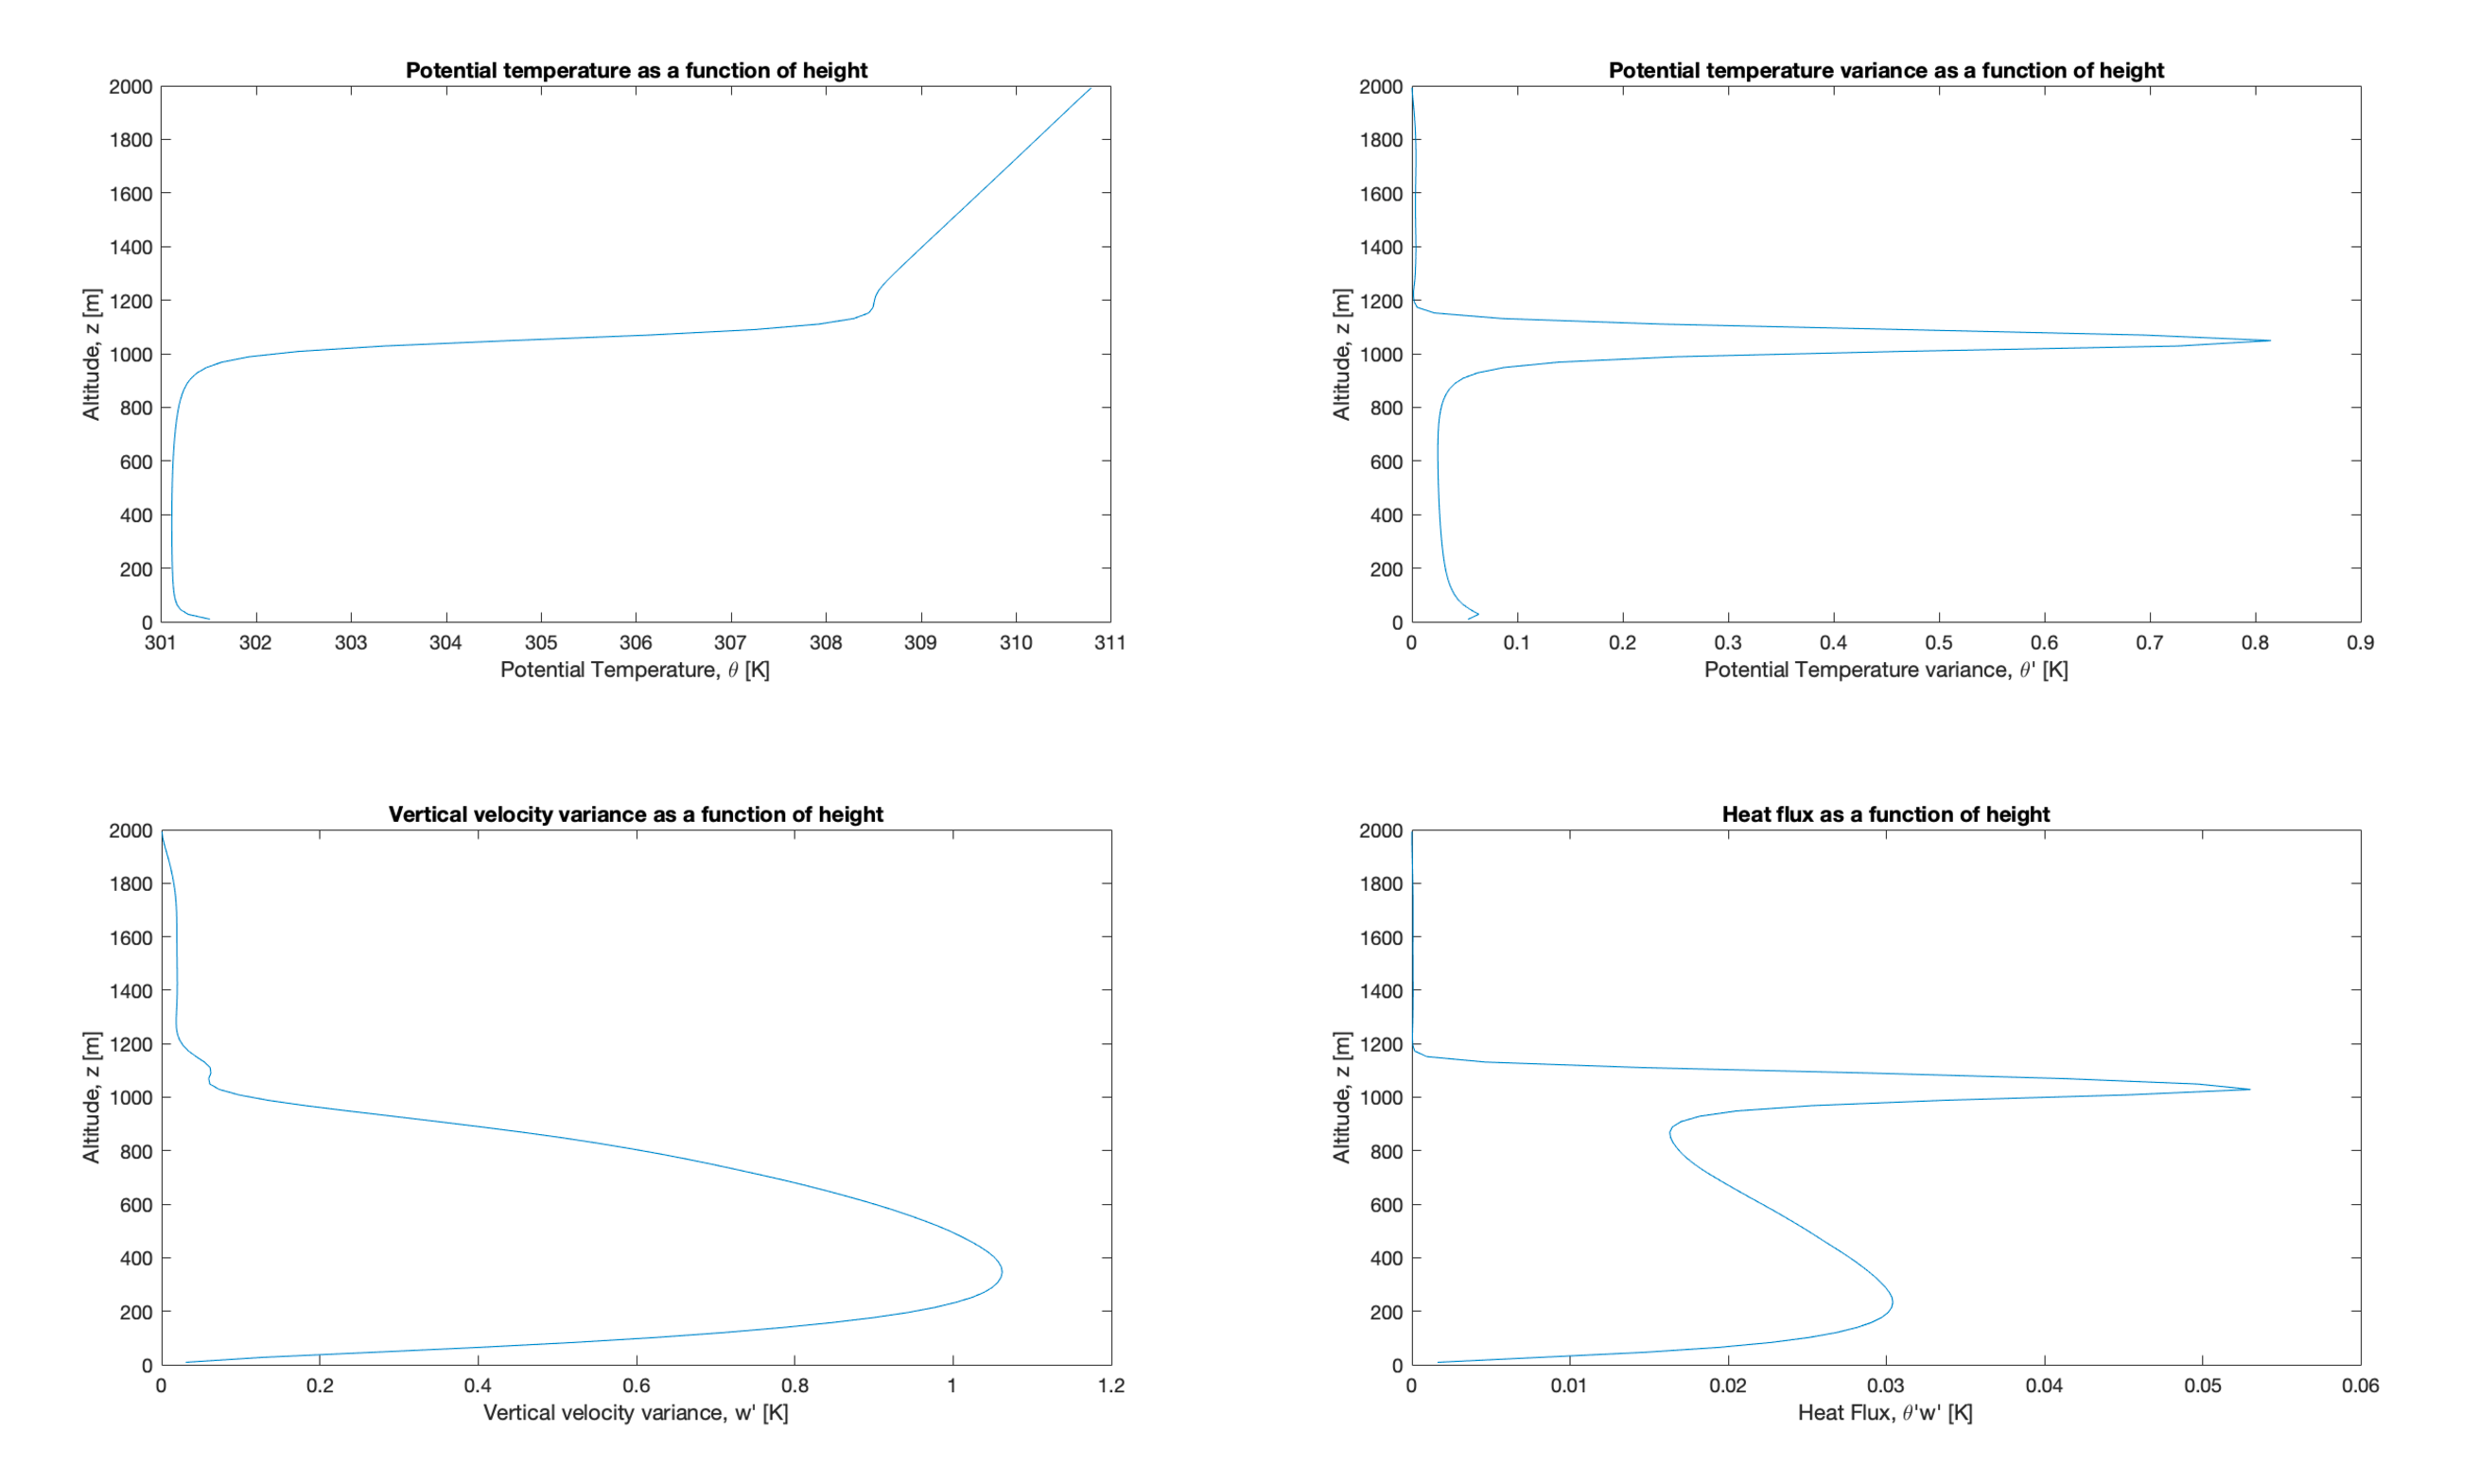
\includegraphics[width=\linewidth]{images/ABL_Vertical_Profiles.pdf}
\end{figure}


\section{Tuesday, March 8, 2022}
\par
To continue on yesterday’s discussion about solid-state propulsion, Barrett’s group used a corona discharge thruster to propel the aircraft. This works by applying a DC voltage across two asymmetric electrodes as shown, where the positive electrode is a wire that ionizes air molecules within some radius, referred to as the corona (is this related to the Debye length?) and the negative electrode is some sort of mesh material. Ionized materials then move along the induced electric field and collide with neutral air molecules to produce in the opposite direction of ion flow. 

\begin{figure}[H]
\centering
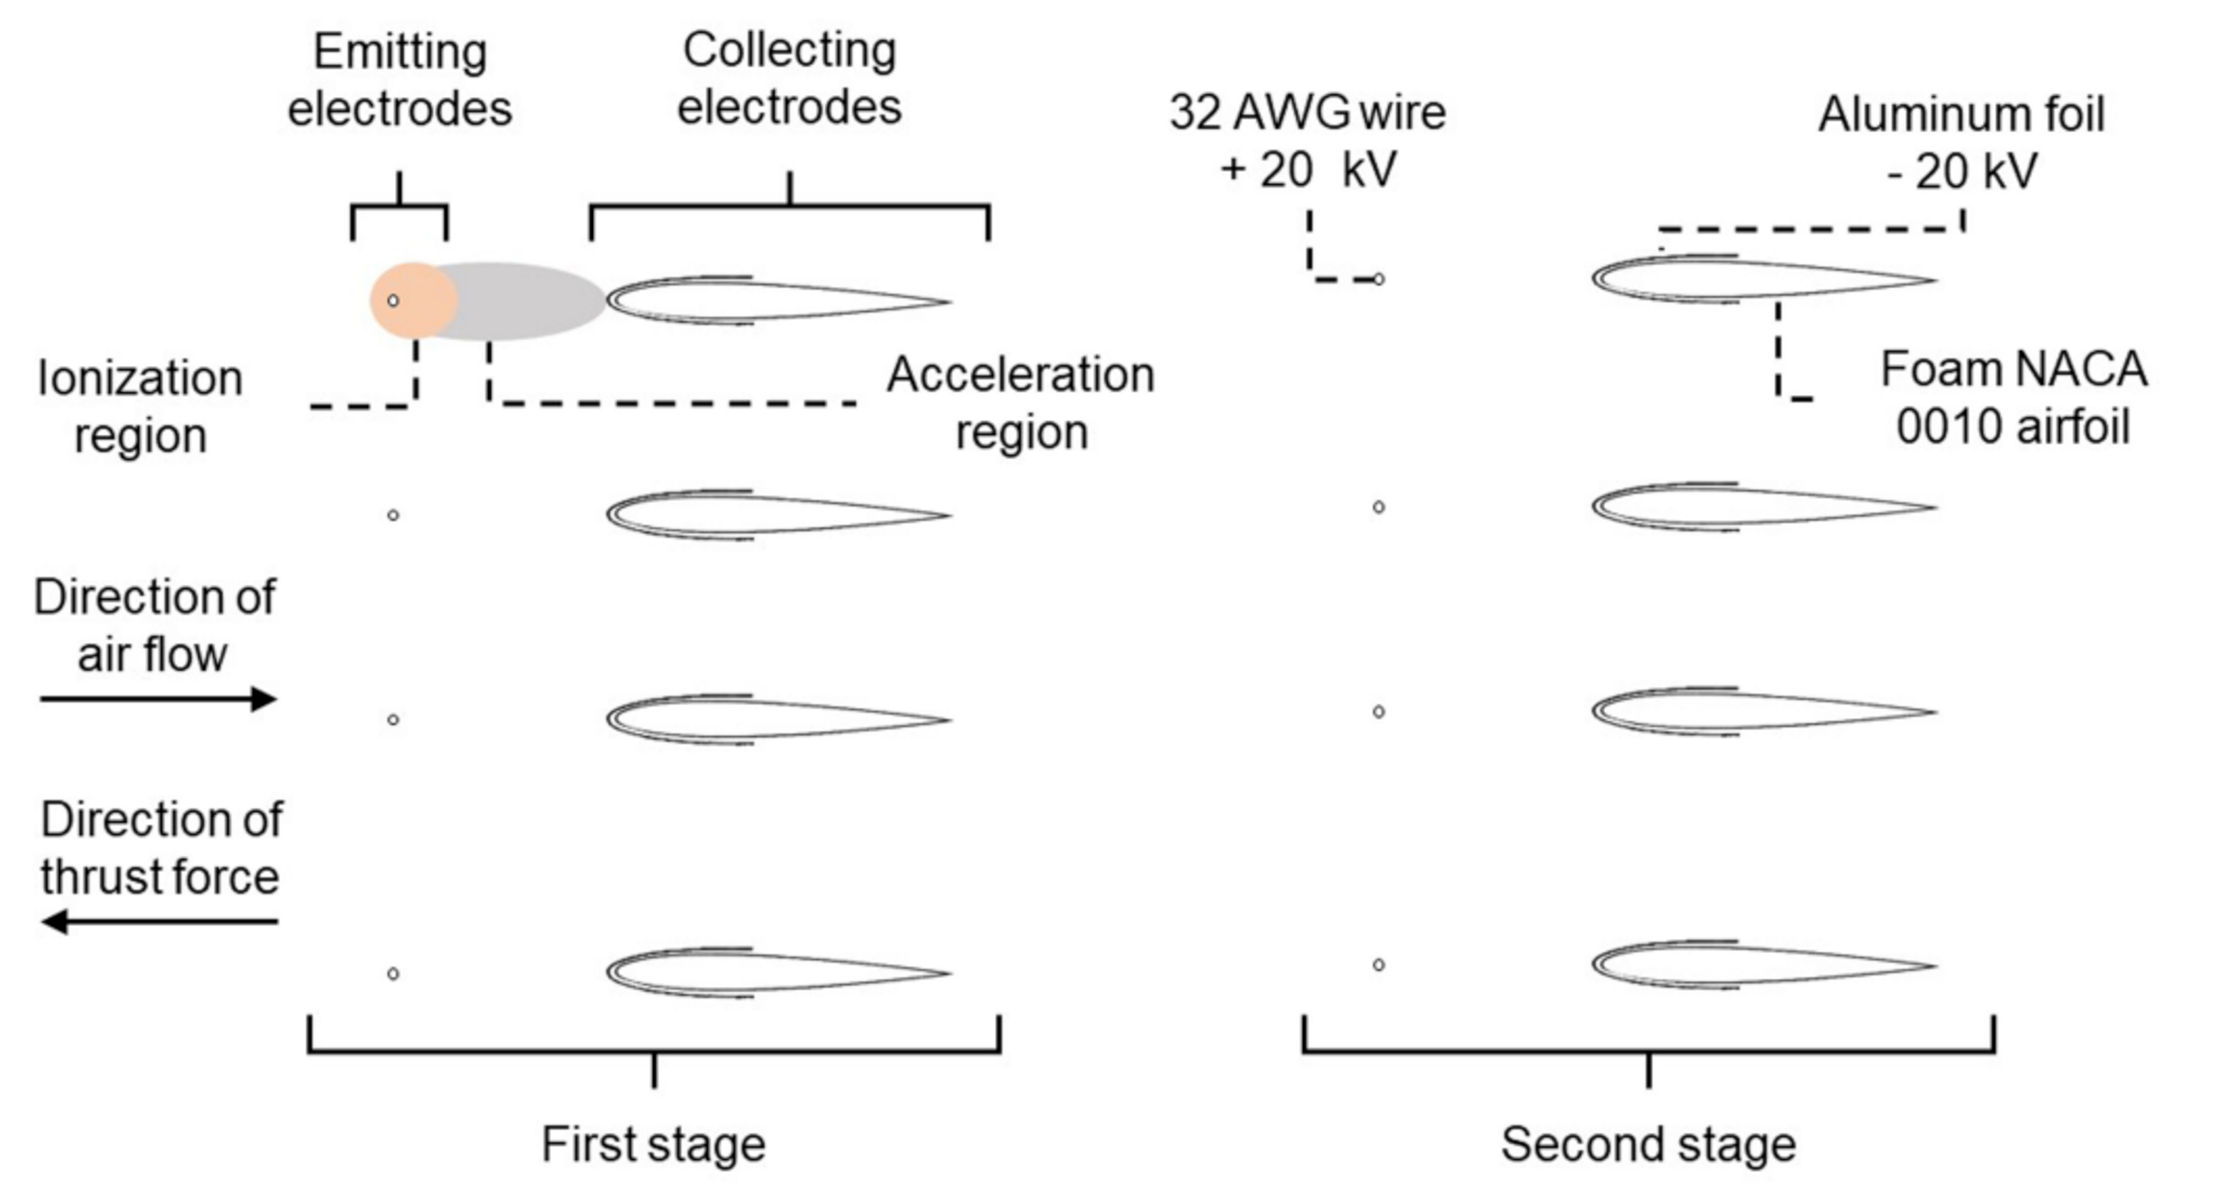
\includegraphics[width=\linewidth]{images/thrustdiagram.pdf}
\end{figure}

\par
However, in their paper, \textit{A dielectric barrier discharge ion source increases thrust and efficiency of electroaerodynamic propulsion}, they note that a corona discharge can be limited by two processes (1) a minimum electric field at the emitter for ionization and (2) a maximum space charge density arising from the self-limiting nature of electric-field driven charge flow. Thus, they proposed a decoupled system using a dielectric barrier discharge plasma where ions are produced by a separate ``emitter." By using a decoupled thrusted more current can be produced and, as a result, more thrust. 

\begin{figure}[H]
\centering
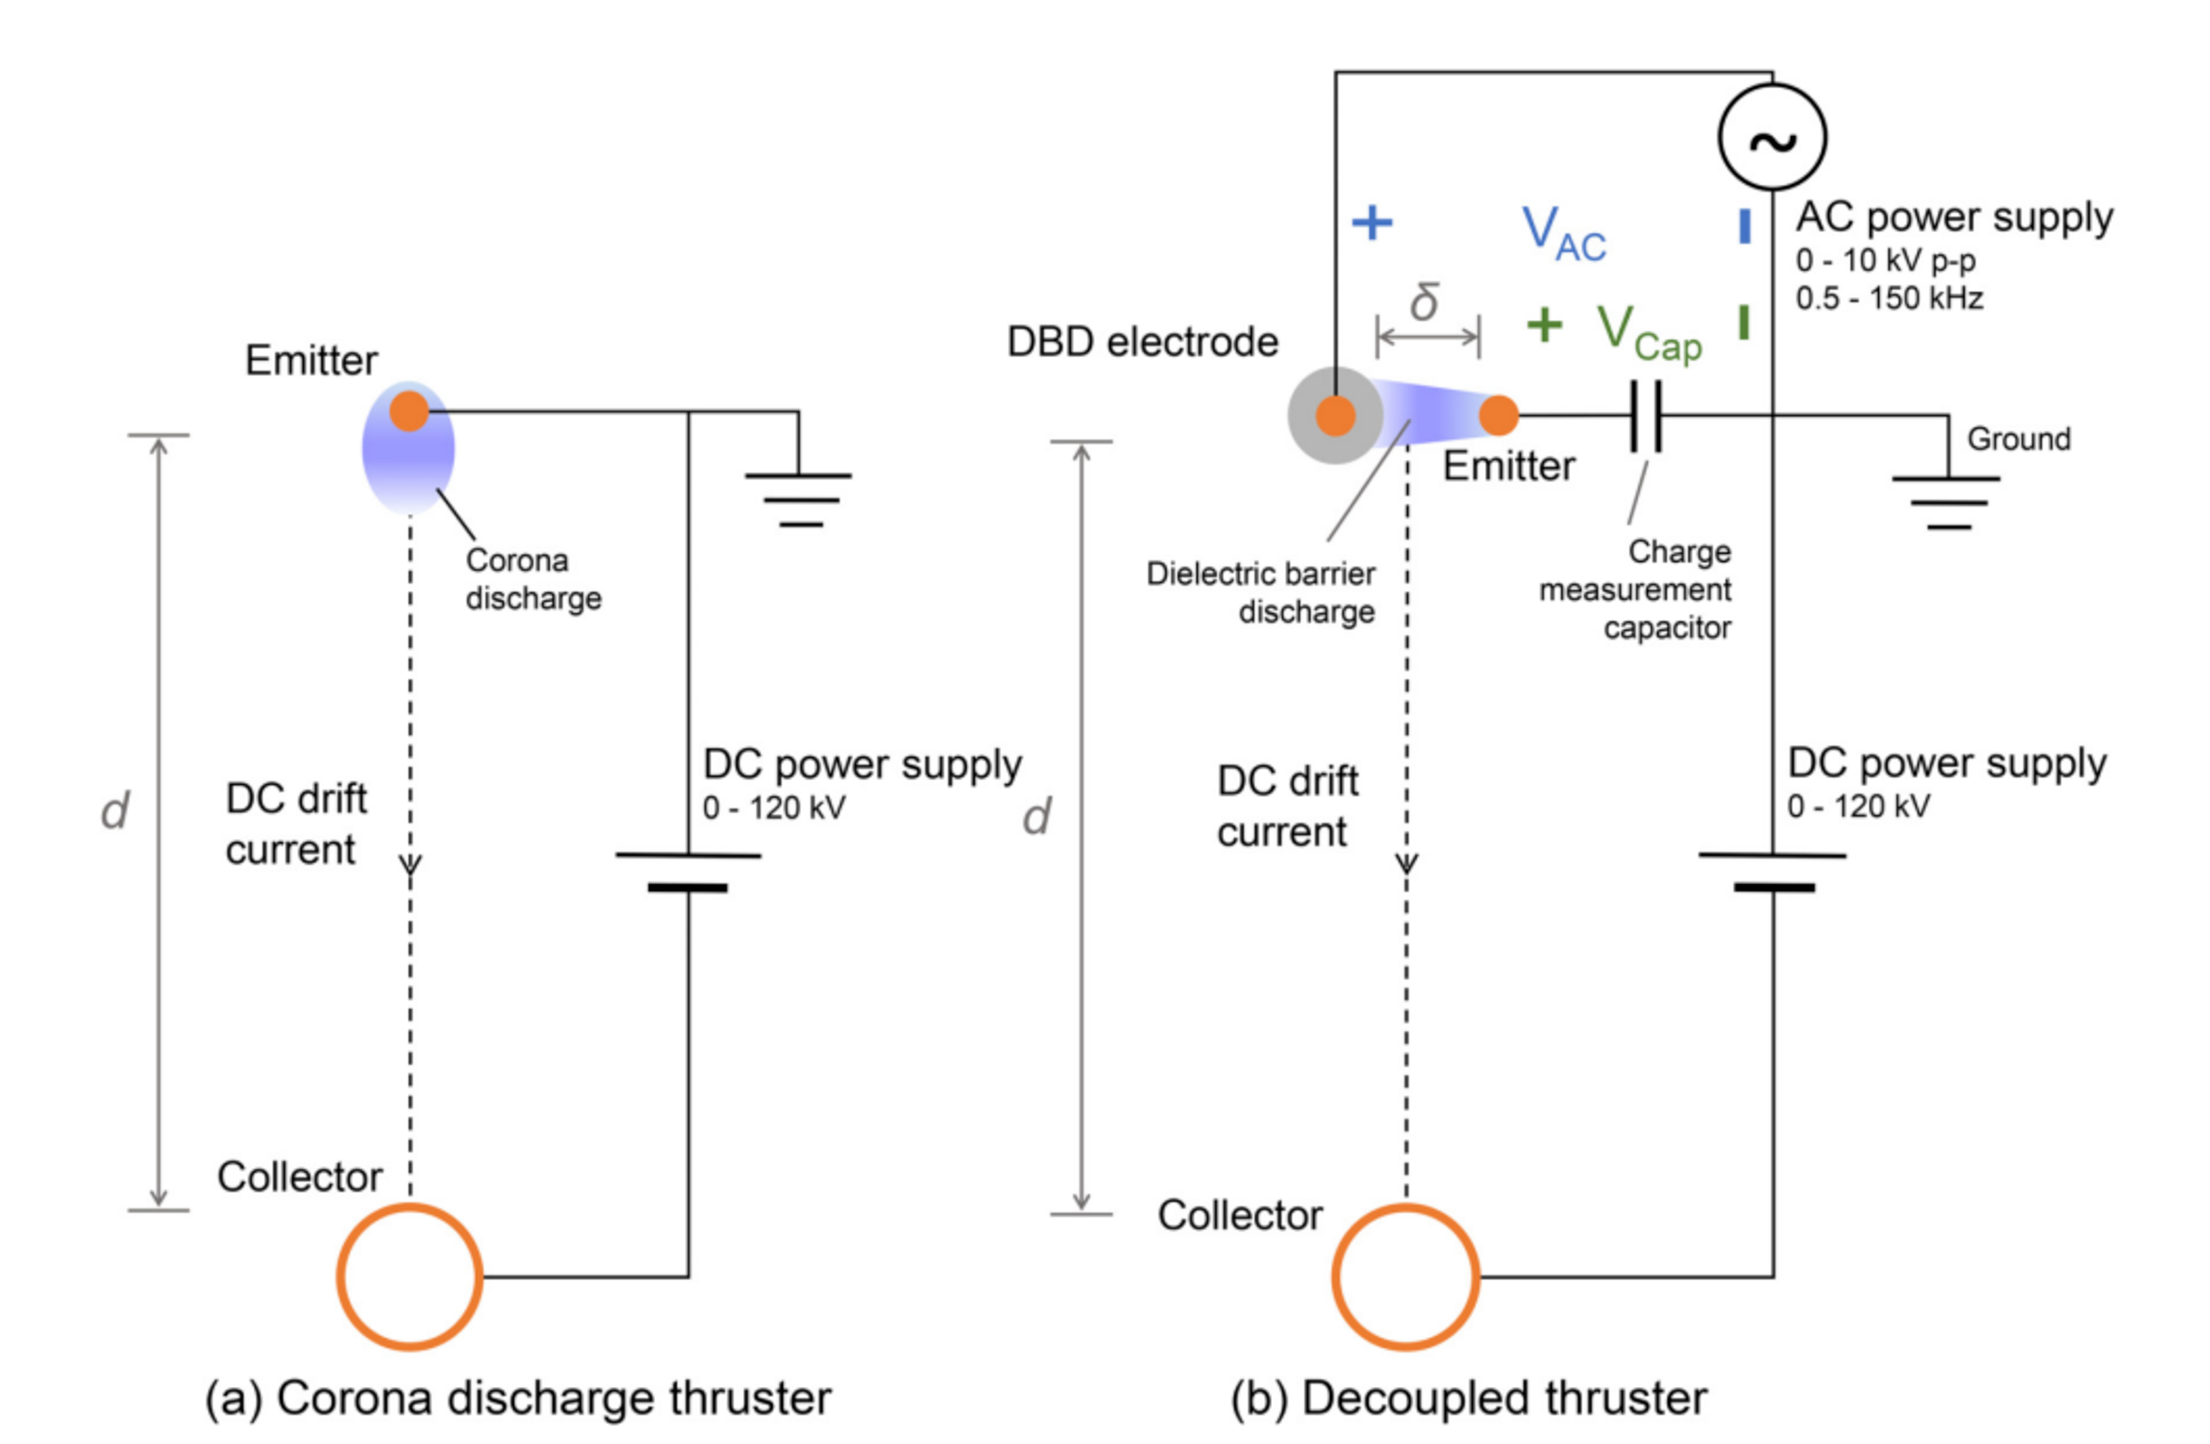
\includegraphics[width=\linewidth]{images/dbd thruster schematic.pdf}
\end{figure}

\section{Monday, March 7, 2022}
\par
An interesting topic that I was reading about today is “ionocraft” which are airplanes propelled by ion propulsion systems that have no moving parts. This article by Steven Barrett’s group shows a proof of concept on how a heavier than air craft can be propelled by ionic wind. From my understanding, it works by using high-voltage electrodes (20 kV+?) to ionize air (mostly N2) and accelerate the ions across the electric field to the negative electrode.  The thrust force is generated as a reaction to the motion of the ions. In their proof-of-concept tests, the craft traveled between 40-45 meters in 8-9s before turning the thruster off.

\begin{figure}[H]
\centering
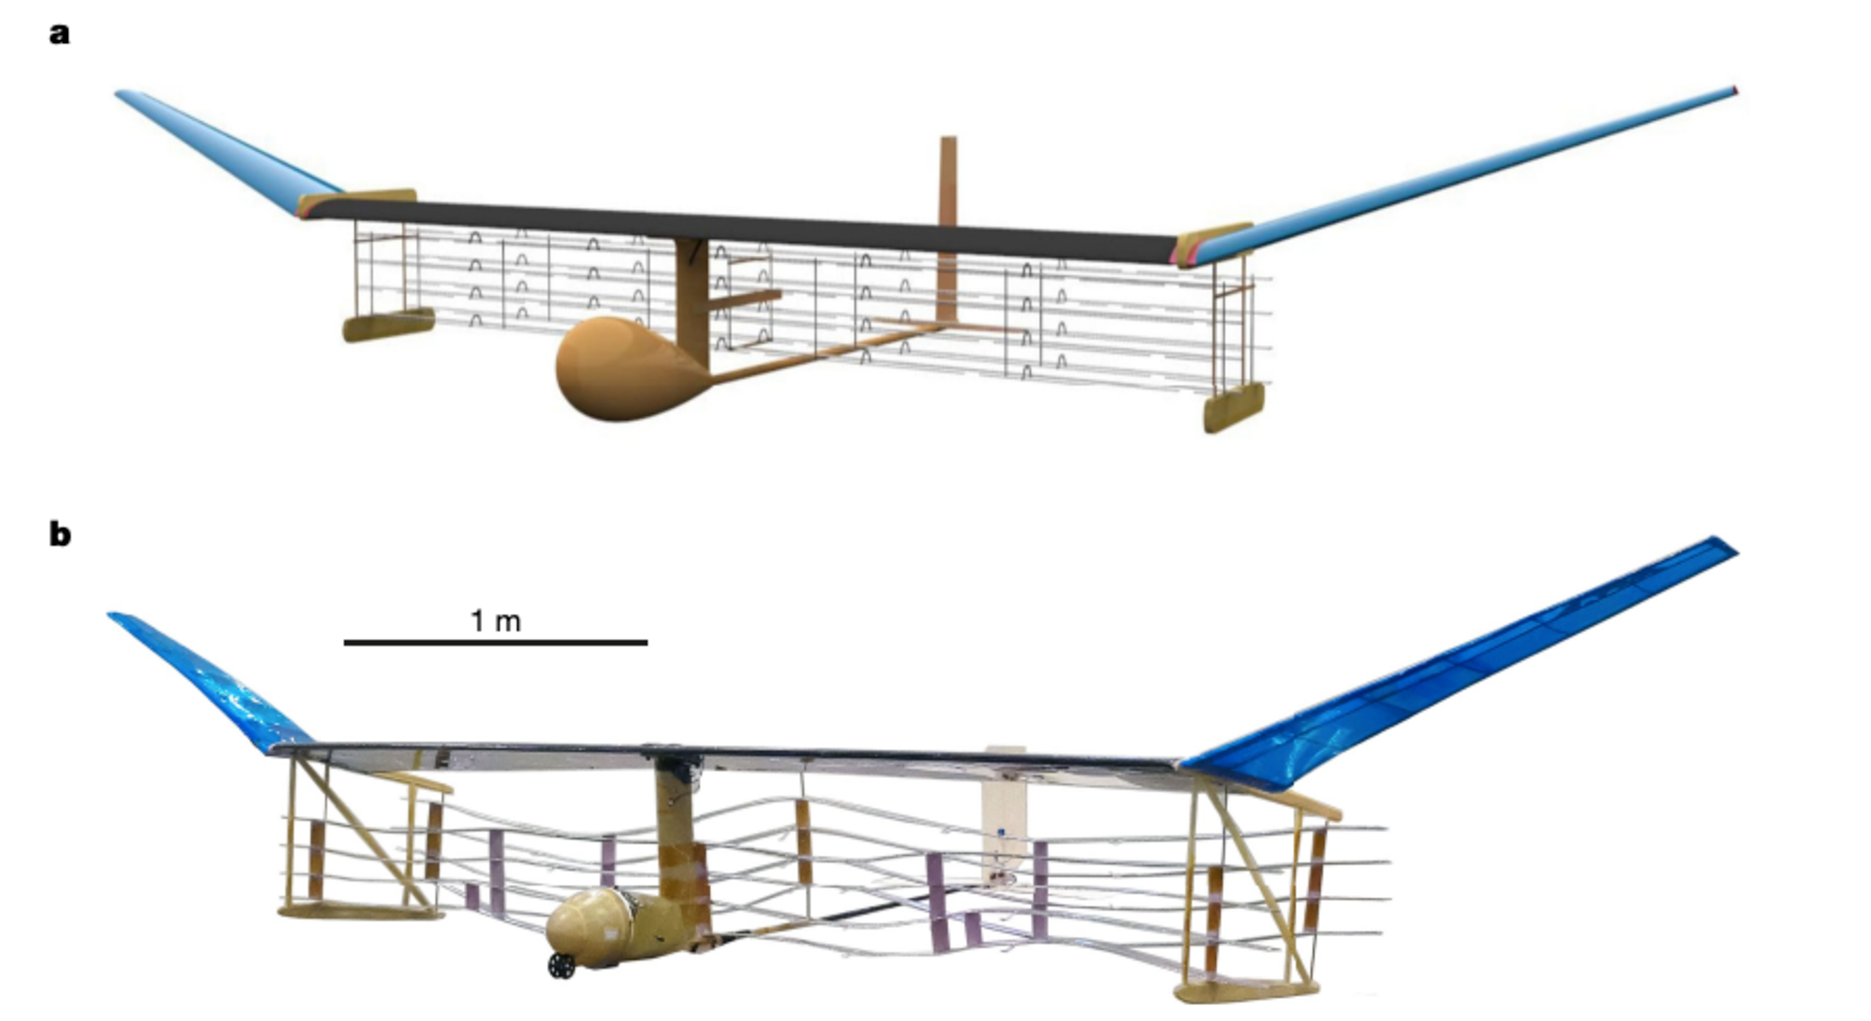
\includegraphics[width=\linewidth]{images/ionicwindplane.pdf}
\end{figure}

\begin{figure}[H]
\centering
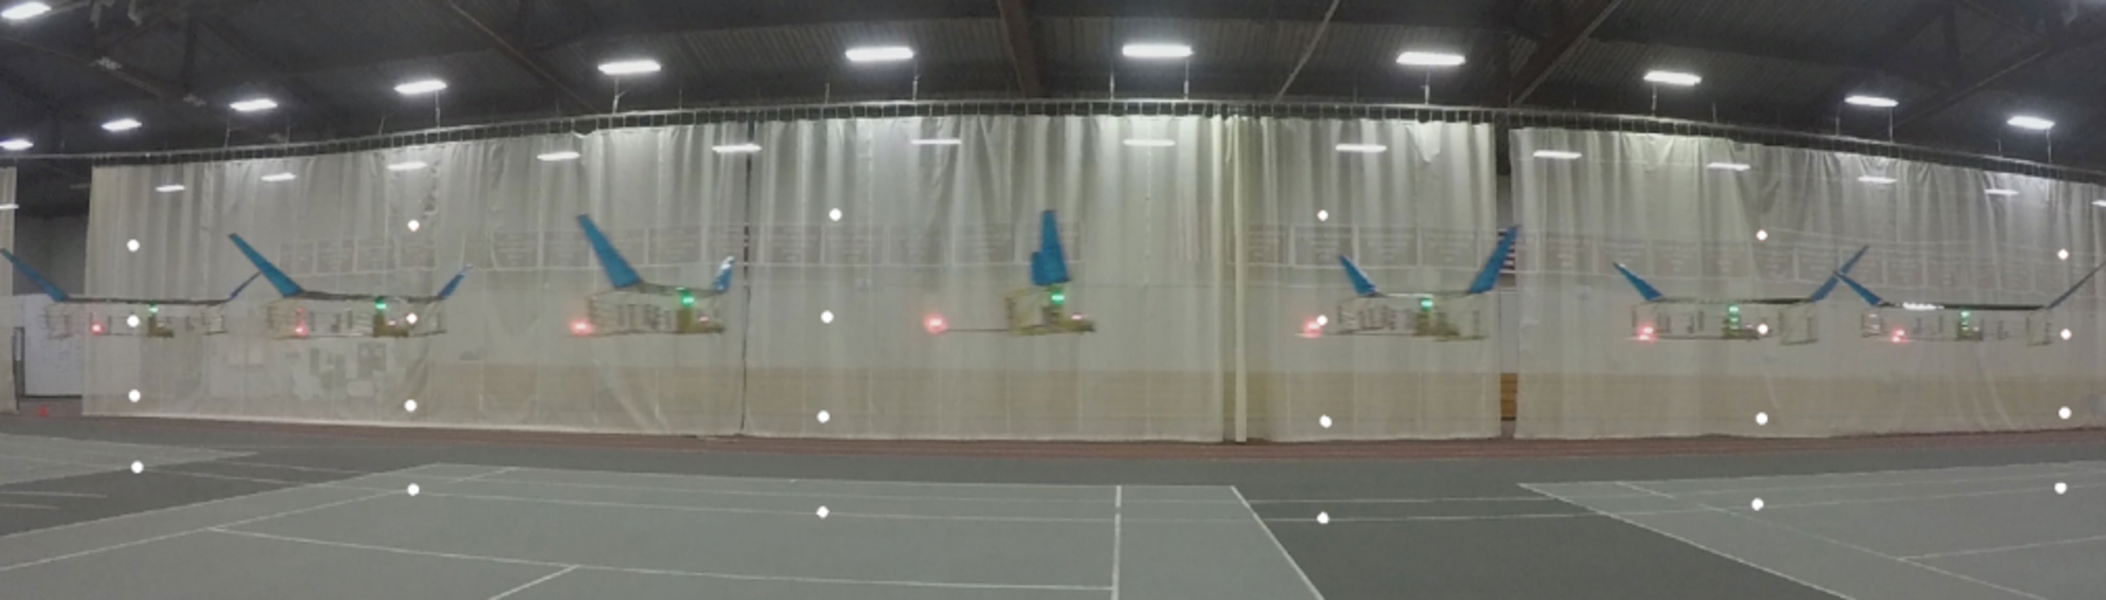
\includegraphics[width=\linewidth]{images/ionocraftmotion.pdf}
\end{figure}

\par
Today I also spent some time working on a computational fluid mechanics problem set for my Physics of Wind course. Given collected over a domain and assuming horizontally homogeneity I spatially averaged the data to study potential temperature and vertical velocity as a function of altitude in the atmospheric boundary layer. One part of the assignment involves applying similarity relationships to estimate the convective velocity scale and the surface heat flux, but I am not exactly sure how to do that. 



\end{document}